% ==============================================================================
% thesis.tex
% Example file for tumthesis.csl
% Michael Ritter, 2012
% Licence:
% This work may be distributed and/or modified under the
% conditions of the LaTeX Project Public License, either version 1.3
% of this license or (at your option) any later version.
% The latest version of this license is in
% http://www.latex-project.org/lppl.txt
% and version 1.3 or later is part of all distributions of LaTeX
% version 2005/12/01 or later.
% ==============================================================================
\documentclass[]{tumthesis}

% ------------------------------------------------------------------------------
%FixMe-Status: final (no FixMe comments) or draft (comments visible)
%\fxsetup{draft}
\fxsetup{final}
% ------------------------------------------------------------------------------

% ------------------------------------------------------------------------------
%  Language selection for metadata and main text (can be changed at any point in
%  the main text.
%\selectlanguage{ngerman}
\selectlanguage{english}
% ------------------------------------------------------------------------------

\def\defSubject{idp}
%working title http://www-m9.ma.tum.de/Allgemeines/WolfgangRiedl

\def\defTitle{Visualization of advanced graph algorithms}% using the example of push-relabel as well as label-setting algorithms}

\def\defTitleDE{Darstellung von fortgeschrittenen Graphalgorithmen}% am Beispiel von Push-Relabel sowie Label-Correcting Algorithmen} %%Setting oder Correcting?


\def\pushRelabel{\texttt{push-relabel algorithm}} %Goldberg-Tarjan
\def\maxflow{\textit{maximum flow problem}}
\def\labelSetting{\texttt{label-setting algorithm}}
\def\spprc{\textit{shortest path problem with resource constraints}}

\def\pushRelabelDE{\texttt{Push-Relabel Algorithmus}} %Goldberg-Tarjan
\def\maxflowDE{\textit{Max-Flow Problem}}
\def\maxflowDEGen{\textit{Max-Flow Problems}}
\def\labelSettingDE{\texttt{Label-Setting Algorithmus}}
\def\spprcDE{\textit{Kürzeste-Wege Problem mit Ressourcenbeschränkungen}}
\def\spprcDEGen{\textit{Kürzeste-Wege Problems mit Ressourcenbeschränkungen}} %genitiv



\def\defSubTitle{
\pushRelabel{} \\ to solve the \maxflow{} \\
\labelSetting{} \\ to solve the \spprc{}
}
\def\defProfessor{Prof. Dr. Peter Gritzmann}
\def\defAdvisor{Wolfgang F. Riedl}
\def\defAuthor{Adrian Haarbach}
\def\defDate{December 30, 2016}
\def\defLocation{Munich}
\input{eqname}


\newcommand{\refSec}[1]{(\cref{#1})}
\newcommand{\refTable}[1]{(\cref{#1})}
\newcommand{\refFigure}[1]{(\cref{#1})}
%\newcommand{\Eqref}[1]{\cref{#1} : \eqnameformat{\nameref{#1}}} %\eqref{#1}
%http://tex.stackexchange.com/questions/156067/suppress-link-or-just-the-color-of-a-specific-nameref
\newcommand{\Eqref}[1]{\eqnameformat{\hypersetup{hidelinks}\nameref{#1}} \eqref{#1}}
\newcommand{\refLine}[1]{(\cref{#1})} %\autoref label{algo:mv-addNodes}

\newcommand{\abs}[1]{\left\lvert#1\right\rvert} % absolute value: single vertical bars
\newcommand{\norm}[1]{\left\|#1\right\|}
\newcommand{\Norm}[1]{\left\lVert#1\right\rVert} % norm: double vertical bars




% ------------------------------------------------------------------------------
% Data for the bibliography
\addbibresource{./contents/resources.bib}
% ------------------------------------------------------------------------------

% ------------------------------------------------------------------------------
% Further packages and TikZ libraries can be incorporated here.
\usetikzlibrary{arrows}
% ------------------------------------------------------------------------------

% ------------------------------------------------------------------------------
% Using the include-command: The content of the work will be incorporated using
% the include-command. So that you can test things out without always needing
% the full thesis, you can define here which sections will be incorporated and
% which will not. Of course, for the final version you should be sure to
% incorporate everything.
%\includeonly{%
%%titlepage,%
%%declaration,%
%abstract,%
%introduction,%
%% include own sections here (rule of thumb: one file per chapter)
%conclusion,%
%appendix%
%}%
% ------------------------------------------------------------------------------

% ------------------------------------------------------------------------------
% PDF-Metadaten
\hypersetup{
 pdfauthor={\defAuthor},
 pdftitle={\defTitle},
 pdfsubject={},%\defSubTitle},
 pdfkeywords={},%\subject{\defSubject}},
 colorlinks=true, %coloured links (for the PDF version)
 %colorlinks=false, % no coloured links (for the print version)
 bookmarksnumbered=true,     
 bookmarksopen=true,         
 bookmarksopenlevel=1,
 pdfstartview=Fit,           
 %pdfpagemode=UseOutlines,    % this is the option you were lookin for
 pdfpagelayout=TwoPageRight,
    pdfborder={0 0 0},
}
% ------------------------------------------------------------------------------

% ------------------------------------------------------------------------------
% Data for the title page and declaration
\author{\defAuthor}
\title{\defTitle}
\subtitle{\defSubTitle}
\faculty{Fakultät für Mathematik}
\institute{Lehrstuhl für Angewandte Geometrie und Diskrete Mathematik}
%\subject{master}
%\subject{bachelor}
%\subject{diploma}
%\subject{project}
%\subject{seminar}
%\subject{idp}
\subject{\defSubject}
\professor{\defProfessor} %Themensteller
\advisor{\defAdvisor} %Betreuer
\date{\defDate}%\today} %Submission Date
\place{\defLocation} %Place where document is signed
% ------------------------------------------------------------------------------

% ==============================================================================
% Main part of the document
% ==============================================================================
\makeindex[title=Index,options=-s myindex]
\begin{document}
\pagestyle{empty}
\frontmatter%
%\selectlanguage{ngerman}
\selectlanguage{english}
\maketitlepage%
\makedeclaration%

%==================================================
% abstract.tex
% Beispieldatei für tumthesis.cls und thesis.tex
% Michael Ritter, 2012
% Lizenz: 
% This work may be distributed and/or modified under the
% conditions of the LaTeX Project Public License, either version 1.3
% of this license or (at your option) any later version.
% The latest version of this license is in
% http://www.latex-project.org/lppl.txt
% and version 1.3 or later is part of all distributions of LaTeX
% version 2005/12/01 or later.
%==================================================
\cleardoublepage

\selectlanguage{english}
\section*{Abstract}
This interdisciplinary project deals with the vivid visualization of advanced graph algorithms. In particular, algorithms to solve two distinctive problems in discrete math are considered. Namely the \texttt{max-flow problem} as well as the \texttt{shortest path problem with resource constraints}.
For efficiency reasons, one often employs advanced graph algorithms to solve above problems. The \texttt{max-flow problem} is solved using the efficient push-relabel algorithm of Goldberg-Tarjan. To solve the \texttt{shortest path problem with resource constraints}, we employ a generic label-setting algorithm which follows the dynamic programming principle.
%This IDP aims at extending the previous HTML5 framework that was developed at the chair to support advanced graph algorithms:
%\begin{itemize}
%	\item the Tarjan-Goldberg push-relabel algorithm to solve the maximum flow problem
%	\item a Label Setting algorithm to solve the shortest path problem with resource constraints (SPPRC)
%\end{itemize}
%In particular, the goal was to provide an intuitive visual representation of all state variables and state transitions during the algorithm execution. Since both algorithms carry a lot of state information, an additional visualization layer, linked to the original graph layer was developed. This second layer displays: 
%\begin{itemize}
%	\item the height function of each node in case of the Tarjan-Goldberg algorithm
%	\item the pareto frontier of all labels resident in a certain node in case of the Label Setting algorithm
%\end{itemize}
%
%To achieve the goal of a highly interactive and easily extensible user experience, we replaced the old canvas based graph visualization code, which was really hard to extend, with a new implementation using the Stanford development D3.js (or just D3 for Data-Driven Documents), a JavaScript library for producing dynamic, interactive data visualizations in web browsers. It makes use of the widely implemented SVG, HTML5, and CSS standards. 
%
%During the development process, we also migrated the existing graph editor to the new technologies, it now easily supportsan arbitrary number of resources defined on edges and nodes download and upload functionality cropped SVG export of graphs
%
%This talk is not only suitable to mathematicians found of graph problems, but to anyone who wants to leverage today's web standards to express his interactive visualization needs.
%

\selectlanguage{ngerman}
\section*{Zusammenfassung}
Das vorliegende interdisziplinäre Projekt beschäftigt sich mit der anschaulichen Darstellung von fortgeschrittenen Graphalgorithmen. Betrachtet werden zwei Verfahren zur Lösung von Problemstellungen der diskreten Mathematik. Die zu visualisierenden Problemstellungen sind hierbei das \texttt{Max-Flow Problem} sowie das \texttt{Kürzeste-Wege Problem mit Ressourcenbeschränkungen}.
Als Lösungsverfahren für die aufgeführten Problemstellungen werden aus Effizienzgründen häufig fortgeschrittene Graphalgorithmen herangezogen. Für die Lösung des Max-Flow Problems findet der bekannte Push-Relabel Algorithmus von Goldberg-Tarjan in der Praxis häufig Anwendung. Zur Lösung des Kürzeste-Wege Problems mit Ressourcenbeschränkungen wird mit einem Label-Setting Algorithmus ein bekanntes Verfahren der dynamischen Programmierung vorgestellt.
%Das interdisziplinäre Projekt hat das Ziel, die erwähnten Problemstellungen mit einfachen Worten zu erklären und durch Beispiele zu motivieren sowie die verwendeten Lösungsverfahren graphisch zu veranschaulichen. Die Darstellung wird hierbei in Form einer separaten Web-Applikation für jede Problemstellung erfolgen, welche aus Gründen der einheitlichen Darstellung und der der leichteren Wartbarkeit auf ein gemeinsames, bereits existierendes Framework aufbauen wird.

\selectlanguage{english}

%%% Local Variables: 
%%% mode: latex
%%% TeX-master: "thesis"
%%% End: 
\tableofcontents%

\mainmatter%
\pagestyle{headings}

\chapter{Introduction}\label{ch:1}

Most previous visualizations of graph algorithms \cite{storz2013idp,velden2014idp,sefidgar2015idp,becker2015idp,zoennchen2015idp,fischer2016idp,feil2016idp} are based on displaying the state of the algorithm on top of a network visualization of a graph, e.g. by annotating vertices or edges with additional information.

For advanced graph algorithms \cite{goldberg1988new,irnich2005shortest}, which are often employed for efficiency reasons, the state size to visualize may become quite large. It may be thus advantageous to visualize the state of such algorithms in an additional visualization layer. 

The ideas of these visualizations have long existed in a static form in textbooks describing the theory behind these algorithms with specific examples. Nevertheless, we are unaware of a dynamic visualization of these additional state variables.

\section{Related work}
The primary sources of the algorithms of this work are \cite{goldberg1988new,irnich2005shortest}. Secondary source for the first algorithm is the review article \cite{goldberg2014efficient} and for the second one three phd theses, a diploma thesis and a journal article \cite{solomon1983vehicle,ziegelmann2001constrained,schlechte2003resource,feillet2004exact,garcia2009resource}.
A deeper understanding of the problems at hand and a broader view of related algorithms was acquired using standard university textbooks \cite{ahuja1993network,cormen2009introduction,jungnickel2013graphs}, where the last one comes from the math domain, the middle one from the computer science domain, while the first one lies somewhere in between. These allow to grasp the connection between \textit{problem} and \textit{algorithm}.
Another important source of inspiration are the web resources such as lecture slides regarding maxflow \cite{mayer2013prakt,mehlhorn2000maximum,williamson2007network,matuschke2016network} and SPPRC \cite{petersen2006label}. The boost C++ library's documentation is a valuable source of information for both algorithms \cite{boost2002push,boost2006rc}. The SPPRC or VRPTW is additionally handled in a nice website \cite{networking2013vehicle}.

The implementation part of this interdisciplinary project is a large-scale refactoring of previous projects \cite{storz2013idp,velden2014idp,sefidgar2015idp,becker2015idp,zoennchen2015idp} over the duration of two years. The most drastical change is the usage of SVG and D3.js instead of a Canvas based visualizations. A beta version of this project already forms the basis of the latest two interdisciplinary projects \cite{fischer2016idp,feil2016idp}.
The needed JavaScript knowledge was acquired in part with the help of \cite{flanagan2011javascript,crockford2008javascript,haverbeke2015eloquent,resig2013secrets,herman2012effective,stefanov2010javascript}. The first one is the definitive reference for javascript, the second one an advanced book about language features to use or to leave out, the third and fourth one a good introduction for beginners. The last two books cover important language aspects and design patterns, in particular scope and closure, prototypal-based inheritance, statics, singletons and code-reuse patterns.
Concerning D3.js \cite{bostock2011d3}, the crucial part one needs to understand is the data join and the enter, update and exit selection, which are nicely explained in two blog posts \cite{bostock2012join,bostock2016general}. The introductory books \cite{murray2013interactive,zhu2013data,meeks2015d3} also give details on how to implement charts as used for the secondary visualization layer .


\section{Contributions}
The contributions of this work are the following:
\begin{itemize}
	\item Two applications to visualize different problems of discrete math, the maximum flow and the shortest path problem with resource constraints. New concepts for secondary visualization layers are developed and implemented.
	\item A complete and very generic rewrite of the basic graph data structure Graph using hashmaps of Grap.Node and Graph.Edge together. Methods to serialize to file and deserialize to load from file are implemented.
	\item A complete rewrite of the graph visualization code using D3.js and SVG instead of Canvas. This is the GraphDrawer class, which should be used as a base class. Customization is easily possible by overwriting methods that will be called from inside of D3.js data join. Any visualization can be saved to disk in png or svg format, for which styles and marker definitions are automatically inlined.
	\item A new Graph Editor with support for modyfing graphs with arbitrary resources easily. An arbitrary number of resources or constraints can be defined on edges or nodes.
	\item A new way to save stateful data of the graph using JSON.stringify, which makes implementing the reverse functionality much easier.
	\item A Logger utility which allows to log algorithm executution messages with up to 3 indentation levels. This is very useful for development, but also for the final algorithm so people can trace the algorithm execution.
	\item A new way to synchronize between the algorithm state (in the sense of a finite state machine), pseudocode lines, and their description using d3.
\end{itemize}

\section{Overview}

\chapter{Background}\label{ch:2}
Problems defined on networks arise in many real-life applications, such as finding the fastest route between two cities or computing the maximum bandwidth of an internet connection. A network can mathematically be represented by a graph. 

\newcommand{\Ein}[1]{\delta^-(#1)}
\newcommand{\Eout}[1]{\delta^+(#1)}
\newcommand{\ein}{{e_{\text{in}}}}
\newcommand{\eout}{{e_{\text{out}}}}

%for algorithms
%\newcommand{\setfont}[1]{\mathcal{#1}}
\newcommand{\setfont}[1]{#1}

%\section{math}
\begin{definition}[simple directed graph]
A graph is an ordered pair $G = (V, E)$ consisting of a vertex (or node) set $V$ and an edge (or arc) set $E$. The unqualified term "graph" usually refers to a \textit{simple} graph which has no multiple edges or self-loop edges. In a \textit{directed graph (digraph)}, $E$ is a set of ordered pairs of vertices, a subset of the cartesian product of vertices, that is $E \subseteq V \times V$. If the graph is simple, each edge $e \in E$ can be uniquely identified by a pair of vertices from $V$, that is $e=(v,w)$ with $v,w \in V$ and $v \neq w$, where $v$ is the start vertex and $w$ is the end vertex of the directed edge or arc $e$ \cite{jungnickel2013graphs}[1.6]. \end{definition}

\begin{figure}
\centering
	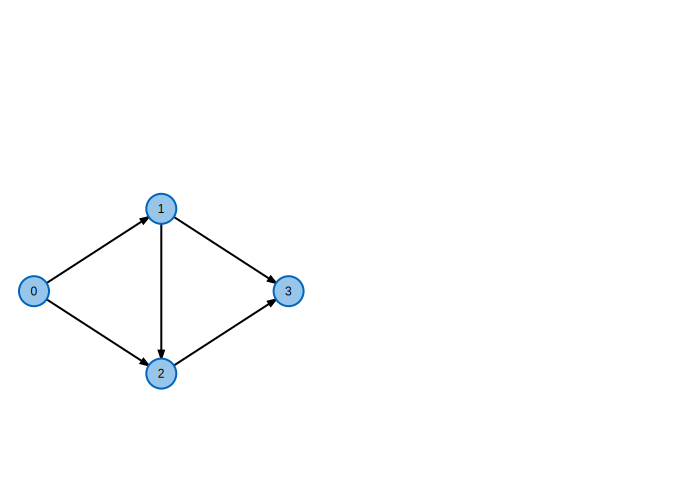
\includegraphics{fig/graph-editor}
	\caption{a digraph with $V=\{0,1,2,3\}$, $E=\{(0,1),(0,2),(1,2),(1,3),(2,3)\}$}
	\label{fig:graph}
\end{figure}

For problems and algorithms defined on digraphs, it is often convenient to define the set of edges coming into a vertex $v$ and zthe set of edges leaving it:
\begin{align}
\Ein{v}  &: \{ e=(u,v) \in E \; | \; u,v \in V \} \tag*{\eqnameformat{incoming edges}} \\
\Eout{v} &: \{ e=(v,w) \in E \; | \; v,w \in V \} \tag*{\eqnameformat{outgoing edges}}
\end{align}
In above example of a digraph \refFigure{fig:graph}, the vertex $v=2$ has an incoming edge set of $\Ein{2}=\{(0,2),(1,2)\}$ and an outgoing edge set of $\Eout{2}=\{(2,3)\}$.

\newpage
%\section{computer science}
Advanced algorithms to solve graph problems rely on common programming principles. The first one is so basic that it actually forms the basis of sorting algorithms such as \texttt{MergeSort}.
\begin{definition}[divide-and-conquer]
\textit{In divide-and-conquer, we solve a problem recursively, applying three steps at each level of the recursion:
\textbf{Divide} the problem into a number of subproblems that are smaller instances of the same problem. 
\textbf{Conquer} the subproblems by solving them recursively. If the subproblem sizes are small enough, however, just solve the subproblems in a straightforward manner. 
\textbf{Combine} the solutions to the subproblems into the solution for the original problem.} \cite[ch. 4]{cormen2009introduction}
\end{definition}

Recursion is clear and appealing from a mathematical perspective, but for computational efficiency reasons, divide-and-conquer is not always the best choice. It is better to remember useful intermediate results.
%\begin{definition}[recurrence]
%A recurrence relation is a mathematical formulation of the divide-and-conquer paradigm, an equation or inequality that descibes a function recursively in terms of base case and 
%\end{definition}

\begin{definition}[dynamic programming]
\textit{Dynamic programming, like the divide-and-conquer method, solves problems by combining the solutions to subproblems. %(“Programming” in this context refers to a tabular method, not to writing computer code.) 
[...] divide-and-conquer algorithms partition the problem into disjoint subproblems, solve the subproblems recursively, and then combine their solutions to solve the original problem. In contrast, dynamic programming applies when the subproblems overlap - that is, when subproblems share subsubproblems. In this context, a divide-and-conquer algorithm does more work than necessary, repeatedly solving the common subsubproblems. A dynamic-programming algorithm solves each subsubproblem just once and then saves its answer in a table, thereby avoiding the work of recomputing the answer every time it solves each subsubproblem.} \cite[ch. 15]{cormen2009introduction} 
%\cite[ch. 3, p. 70]{ahuja1993network}
\end{definition}
Dynamic programming can be applied to a wide range of graph problems, as we will see later. It works because of Bellman's:
\begin{definition}[Principle of Optimality]
\textit{An optimal policy has the property that whatever the initial state and initial decision are, the remaining decisions must constitute an optimal policy with regard to the state resulting from the first decision} \cite[sec. 3.3]{bellman1957dynamic}.
\end{definition}

For some kind of problems, we can get even more efficient with the greedy approach originating from matroid theory \cite[sec. 13.7, p. 528]{ahuja1993network} \cite[ch. 5]{jungnickel2013graphs}. It is at the heart of the efficient and well known Dijkstra algorithm.
\begin{definition}[greedy]
\textit{Algorithms for optimization problems typically go through a sequence of steps, with a set of choices at each step. For many optimization problems, using dynamic programming to determine the best choices is overkill; simpler, more efficient algorithms will do. A greedy algorithm always makes the choice that looks best at the moment. That is, it makes a locally optimal choice in the hope that this choice will lead to a globally optimal solution.} \cite[ch. 16]{cormen2009introduction}
\end{definition}

\chapter{Maximum flows}\label{ch:3}

\section{The \maxflow{}}
An important problem in many applications is to find out the maximum amount of flow that can simultaneously be transferred over a network between two points. % from $s$ to $t$. 
Depending on the context, flow can mean different things, e.g the amount of water in a water pipe system in your city or the bandwidth of a computer network. We call such a network a \textit{flow network}:

\begin{definition}[flow network]
A \textit{flow network} $N$ is a 4-tuple $N=(G,c,s,t)$ consisting of a \textit{digraph} $G$, a positive real-valued capacity function $c: E \rightarrow \mathbb{R}_+ , \forall e \in E : c(e) \geq 0$ defined on all edges of the graph and two designated vertices, the \textit{source} $s \in V$ and the \textit{sink} (or target) $t \in V$ \cite{ahuja1993network}[1.2].
\end{definition}


%However, the links in the network on paths from $s$ to $t$ can only handle flow up to their maximum capacity $c$. One now seeks an assignment of flow values $f$ to edges $e$ that fulfills all the capacity constraints of the edges and the flow conservation property on all the inner nodes, meaning we don't want leaks in our pipe system.
However, the individual links in the network can only handle flow up to their maximum capacity, e.g. they are limited by the diameter of the water pipe. Additionally, the total flow must be preserved at the intermediate joints, e.g. we don't want leaks in our pipe system. This is called a \textit{feasible flow}:% Given such a network, an obvious problem is to find out the maximum amount of flow that can simultaneously be transfered over the network, 


\begin{definition}[feasible flow]
A \textit{feasible flow} $f$ from $s$ to $t$ is a mapping $f : E \rightarrow \mathbb{R}$ satisfying two constraints: The \Eqref{eq:cap} ensures that the flow over an edge is always positive and not exceeding the edge's maximum capacity, while the \Eqref{eq:conserv} assures that the total flow into a vertex $v \notin {s,t}$ equals the total flow out of $v$:
\begin{align}
0 \leq f(e) \leq c(e) & \forall e \in E \eqname*[eq:cap]{capacity constraint} \\
\sum_{e \in \Ein{v}} f(e) = \sum_{e \in \Eout{v}} f(e) & \forall v \in V \setminus \{s,t\} \eqname*[eq:conserv]{flow conservation} \\ \nonumber
\end{align}
\end{definition}

There might be many feasible flows (e.g the zero flow $f = 0 \, \forall e \in E$), but we are especially interested in transferring as much as possible across the network, the \textit{maximum flow}:
\begin{definition}[maximum flow and flow value]
A \textit{maximum flow} $\max \abs{f}$ is a \textit{feasible flow} that maximizes the \textit{flow value} $\abs{f}$, the amount of flow which flows from $s$ to $t$. This is the net flow into the sink $t$ or out of the source $s$:
\begin{align}
\abs{f} = \sum_{e \in \Ein{t}} f(e) = \sum_{e \in \Eout{s}} f(e) \eqname*[eq:flowval]{flow value} \\ \nonumber
\end{align}
\end{definition}


An important concept in the context of flow algorithms is the residual network capturing possible change to $f$, defined by the residual capacities $c'$ and the \textit{residual graph} $G'$:
\begin{definition}[residual graph]
For a flow $f$ in $G=(V,E)$, we can construct the \textit{residual graph} $G' = (V,E')$ by copying all the vertices $v \in V$ from $G$ and for each $e \in E$ adding one or two edges $e'$ to $E'$ with \textit{residual capacity} $c'$ under the following rules \refFigure{fig:residual}:
\begin{description}
\item[forward edge] if $f(e) < c(e)$ for an edge $e=(a,b) \in E$, then add the forward edge $e' = (a,b)$ with residual capacity $c'(e') = c(e) - f(e)$ to $E'$.
\item[backward edge] if $f(e) > 0$ for an edge $e=(a,b) \in E$, then add the backward edge $e' = (b,a)$ with residual capacity $c'(e') = f(e)$ to $E'$.
\end{description}
\end{definition}

\begin{figure}
\centering
\includegraphics[]{fig/residual}
\caption{Construction of the residual graph $G'$ \cite{mayer2013prakt}.}
\label{fig:residual}
\end{figure}

\clearpage
\section{The \pushRelabel{}}
An early way to compute a maximum flow on a directed graph was called the augmenting path method by Ford-Fulkerson \cite{ford1956maximal}.\footnote{explained in textbooks \cite[sec. 6.4]{ahuja1993network}, \cite[sec. 26.2, p.724]{cormen2009introduction}, \cite[sec. 6.1]{jungnickel2013graphs}} A path with available capacity is an augmenting path, an s-t path in the residual graph. As long as such paths exist, one can increase the flow globally on these paths. If the method terminates, it computes a maximum flow. It is called a method and not an algorithm because the way to find augmenting paths in the residual graph is not fully specified. Furthermore, there is no guarantee on termination and runtime. About 15 years later, two algorithms based on the augmenting path method were developed. They ensure a polynomial time bound by augmenting flow along the shortest path first. The algorithm of Edmonds-Karp \cite{edmonds1972theoretical}\footnote{explained in textbooks \cite[sec. 26.2, p. 727]{cormen2009introduction}, \cite[sec. 6.2]{jungnickel2013graphs}} ensures a runtime of $O(|V|\cdot|E|^2)$ while the one of Dinic \cite{dinic1970algorithm}\footnote{explained in textbooks \cite[sec. 7.4]{ahuja1993network}, \cite[sec. 26.2]{cormen2009introduction}, \cite[sec. 6.4]{jungnickel2013graphs}} improves on that with a runtime of $O(|V|^2\cdot|E|)$. This class of algorithms based on the Ford-Fulkerson method of augmenting paths has been visualized in a previous interdisciplinary project \cite{fischer2016idp}.

Still about another 15 years later, an alternative and more efficient method which uses local operations based on the concept of a preflow and a height function was published: The push-relabel algorithm of Goldberg-Tarjan \cite{goldberg1988new}. In contrast to the previous, less efficient algorithms based on augmenting paths, it changes the flow locally and only needs to construct the residual graph locally. 

\subsection{Excess and height}
The increased efficiency comes at the cost of not maintaining a \textit{feasible flow} during algorithm execution. Instead, a \textit{preflow} is maintained:
\begin{definition}[excess and preflow]
	The \textit{preflow} $\tilde f$ is a generalization of the flow $f$. The \Eqref{eq:cap} of the edges is still maintained, but the \Eqref{eq:conserv} at the vertices is not: The equality sign $=$ is replaced with $\geq$: $\sum_{e \in \Ein{v}} f(e) \geq \sum_{e \in \Eout{v}} f(e) \forall v \in V \setminus \{s\}$.
%This means that more flow can enter an inner node than leaving it, e.g. we allow leaks in our pipe system.
One allows flow \textit{excess}, that is, some vertices can have more incoming than outgoing flow at the intermediate stages of the algorithm \cite{goldberg2014efficient}.  The excess flow at a node $v$ due to the preflow is non-negative for all nodes except for the start node and defined as:
	\begin{align}
		e(v) = \sum_{e \in \Ein{v}} f(e) - \sum_{e \in \Eout{v}} f(e) \geq 0 \quad \forall v \in V \setminus \{s\} \eqname*[eq:excess]{excess} \\ \nonumber
	\end{align}
\end{definition}

\begin{definition}[active node]
As long as a vertex has positive (non-null) excess, it is called an \textit{active node}.
\end{definition}


\begin{remark}
An s-t preflow without active nodes is an s-t flow \cite{matuschke2016network}.	
\end{remark}

Intuitively, we should try to push the excess at a node towards the sink, but what does that mean? Another important concept in the push-relabel algorithm is the height function, which is an approximation of a node's distance to the sink. The local \textit{push} operations try to move \textit{excess} at inner nodes 'downwards' towards the sink. If the current node is at a local minimum and still has excess, we \textit{relabel} the node by increasing its \textit{height} so that subsequent push operations can remove the excess.
\begin{definition}[height, valid labeling]
A \textit{height} function\footnote{also called distance labeling or level function} $h(v) \geq 0 \quad \forall v \in V$ is defined for all vertices of the graph. It is a \textit{valid labeling} of the nodes if it satisfies 
\begin{align}
h(t)=0, h(s)=|V| \quad \text{and} \quad h(v)\leq h(w)+1 \, \forall e'=(v,w) \in E' \eqname*[eq:height]{height} \\ \nonumber	
\end{align}
\end{definition}

\begin{definition}[eligible edge] %or valid with respect to the current height function, 
An edge $e'=(v,w) \in E'$ of the residual graph $G'$ is \textit{eligible} if $h(v)=h(w)+1$, meaning that the current node is one level above the one to where we wish to push excess to.
\end{definition}

\subsection{Termination and runtime}
The important property of the push-relabel algorithm is that when the algorithm terminates, the computed preflow is actually a flow. \textit{This is because there can be no augmenting path from s to t in the residual graph since any such path must contain a steep edge (since s is on level $|V|$, $t$ is on level $0$)} \cite{mehlhorn2000maximum}.

The proof of the runtime involves counting the number of possible saturating and nonsaturating push operations as well as relabel operations. Depending on the way the vertices are selected we get different runtimes, proof sketches in \cite{mehlhorn2000maximum,williamson2007network,matuschke2016network}:
\begin{itemize}
	\item Generic (arbitrary selection rule) with runtime $O(|V|^2 \cdot |E|)$ explained and proved in \cite[sec. 7.6]{ahuja1993network}, \cite[sec. 26.4]{cormen2009introduction}, \cite[alg. 6.6.1]{jungnickel2013graphs}. 
	\item Relabel-To-Front (FIFO selection rule) with runtime $O(|V|^3)$ explained and proved in \cite[sec. 7.7]{ahuja1993network},\cite[sec. 26.5]{cormen2009introduction}, \cite[alg. 6.6.14]{jungnickel2013graphs}.
	\item Highest label selection rule with runtime $O(|V|^2\sqrt{|E|})$ explained and proved in \cite[sec. 7.8]{ahuja1993network} \cite[alg. 6.6.16]{jungnickel2013graphs}.
\end{itemize}

We implemented the Relabel-To-Front variant with the first-in-first-out (FIFO) selection rule. In this variant, a node with excess flow stays active either until a non-saturating push or a relabel occurred. 

\clearpage
\subsection{Pseudocode}
%\documentclass[a4paper,11pt]{article}
%\usepackage[linesnumbered,ruled,vlined]{algorithm2e}
%%\newcommand{\setfont}[1]{\mathcal{#1}}
%\newcommand{\setfont}[1]{#1}
%\begin{document}

\begin{algorithm}[h!]
\caption{Goldberg-Tarjan Push-Relabel algorithm with FIFO selection rule}
\DontPrintSemicolon
\KwIn{digraph $G=(V,E)$ with nodes $s,t \in V$ and edge capacities $c(e) \, \forall e \in E$
%\begin{itemize}
%	\setlength\itemsep{0pt}
%	\setlength{\parskip}{0pt}
%	\item nodes start $s \in V$, sink $t \in V$
%	\item edge capacities $c(e) \, \forall e \in E$
%\end{itemize}
}
\KwOut{A feasible maximum s-t flow f(e)}\vspace{0.2cm}
(* Initialize the preflow *)\;
\ForAll{$e=(u,w) \in E$}{
	$f(e) \gets (u==s) \; ? \; c(e) : 0$\;
	\If{$u==s$ AND $w \neq t$}{$Q$.add(w)}
}
((* Initialize the height function *))\;
$h(s) \gets |V|$\;
\ForAll{$v \in V \setminus \{s \}$}{
	$h(v) \gets$ number of arcs on shortest v-t path\;
}
((* Main Loop *))\;
\While{$\setfont{Q} \neq \emptyset$}{
	$v \gets \setfont{Q}$.pop()\;
	\While{$e(v)>0$ AND $\exists \, e'=(v,w) \in E' \, | \, h(v)==h(w)+1$}{
		(* Push *)\;
		push $\min(e(v),c'(e'))$ flow from v to w\;
		\If{$w \neq s,t$ AND $w \notin \setfont{Q}$}{
			$\setfont{Q}$.add($w$)\;
		}
	}
	\If{$e(v)>0$}{
		(* Relabel *)\;
		$h(v) \gets 1 + \min(\{h(w) | e^*=(v,w)\in E'\})$ \;
		$\setfont{Q}$.add($v$) \;
	}
}
\end{algorithm}


%\end{document}
The pseudocode is split into blocks each consisting of a few lines to form different states of the algorithm that can be visualized. This basically transforms the algorithm into a finite state machine, which was first observed in another recent interdisciplinary project \cite{feil2016idp}. The different states are: 1. INITPREFLOW (lines 1-5), 2. INITHEIGHT (lines 6-9), 3. MAINLOOP (lines 10-12), 4. ADMISSIBLEPUSH (line 13), 5. PUSH (lines 14-14), 6. ADMISSIBLERELABEL (line 18) and 7. RELABEL (lines 19-21). For the detailed description of these states we refer to our web application.

 
\clearpage
\subsection{Visualization concept}
\textit{The crucial requirement is [...] $h(v) = h(w) + 1$. Thus we are only allowed to push along [eligible] residual edges $e'=(v,w)$ for which $h(v)$ is exactly one unit larger than $h(w)$ [...]. We may visualize this rule by thinking of water cascading down a series of terraces of different height, with the height corresponding to the labels. Obviously, water will flow down, and [the eligible edge] condition has the effect of restricting the layout of the terraces so that the water may flow down only one level in each step} \cite[sec. 6.6]{jungnickel2013graphs}.

In our visualization concept \refFigure{fig:maxflow}, we show how excess flow $e(v)$ is pushed downwards the terraces of different height $h(v)$. The primary visualization layer displays the graph network, the capacity of an edge and its current flow value. The secondary visualizaiton layer allows to arrange the graph nodes in a 2-dimensional chart, where the axis can be chosen to be y/x (the usual graph), height/id (so that no nodes overlap) or height/excess. The algorithm switches between the different axes depending on the current state.\footnote{The axes can also be kept fixed based on a user request from TU Ilmenau \url{https://github.com/adrelino/idp-graph-algorithms/commit/4f145861dfba5f8305a24c0f9cc4263cf2b17dcf}}

\begin{figure}
\centering
\begin{subfigure}[t]{0.45\textwidth}
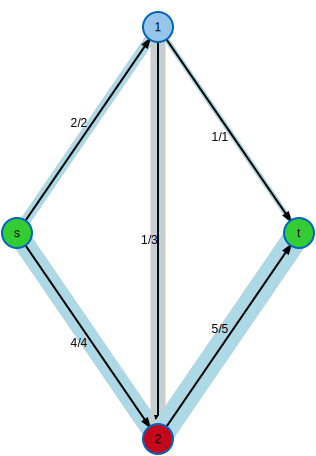
\includegraphics[width=\textwidth]{fig/maxflow-graph-algorithm-graph}
\end{subfigure}
\begin{subfigure}[t]{0.45\textwidth}
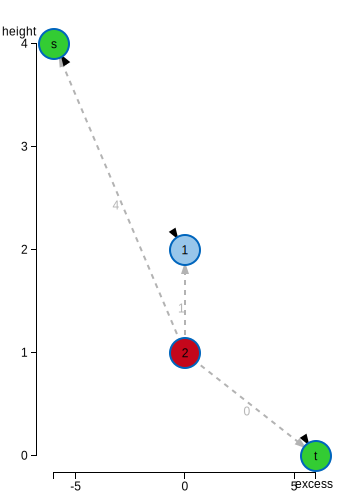
\includegraphics[width=\textwidth]{fig/maxflow-graph-algorithm-height}
\end{subfigure}
\caption{Maxflow concept : The primary visualization layer (left) shows the graph network, with vertices as circles and edges as lines connecting them. Source and target node are coloured in green, the current node in red. The labels of the edges denote the current flow and the maximum capacity in the form flow/cap. The capacity is furthermore drawn as a thick gray line with a width corresponding to its capacity, and the flow is drawn on top of it as a thick blue line. The secondary visualization layer (right) shows the outgoing edges $e'$ of the current node in the residual graph with dashed lines. The nodes are currently arranged according to the height/excess coordinate system axes.}
\label{fig:maxflow}
\end{figure}






\chapter{Visualization Concept}\label{ch:4}
\chapter{Implementation}\label{ch:5}

\newenvironment{ssfont}{\fontfamily{lmss}\selectfont}{\par}

The implementation is an evolution of previous web applications for the visualization of graph algorithms \cite{storz2013idp,velden2014idp,sefidgar2015idp,becker2015idp,zoennchen2015idp}. However, the requirements for graphs with arbitrary resources, a secondary visualization layer and high interactivity urged us to reimplement large parts of the existing codebase using different technologies while still maintaining the same look and feel. In the process, a complete understanding of the interplay between the different components was acquired, which allowed us to refactor them systematically. We improved code quality and maintainability by adhering to object oriented programming best practices of \textit{high cohesion and low coupling} \refFigure{fig:coh}. The separation of the components now fits the \textit{Model-View-Controller (MVC)} design pattern \refFigure{fig:mvc}, which was already applied partially in previous work, even better. 
\begin{figure}
\centering
\begin{subfigure}[b]{0.3\textwidth}
\includegraphics[width=\textwidth]{fig/MVC-Process}
	\caption{Model-View-Controller(MVC)\footnotemark}
	\label{fig:mvc}
\end{subfigure}
\begin{subfigure}[b]{0.68\textwidth}
\begin{small}
\begin{ssfont}
\begin{itemize}
\item Cohesion refers to the degree to which the elements of a class belong together, suggestion is all the related code should be close to each other, so we should strive for \textbf{high cohesion} and bind all related code together as far as possible. It has to do with the elements \textit{within} the class. %\textbf{High cohesion} means a class should do only one thing, but very well.
\item Coupling refers to the degree to which the different classes depend on each other, suggestion is all modules should be independent as far as possible, that's why \textbf{low coupling}. It has to do with the elements \textit{among} different classes. %\textbf{low coupling} suggest that class should have least possible dependencies.
\end{itemize}
\end{ssfont}
\end{small}
\caption{high cohesion, low coupling\footnotemark}
\label{fig:coh}
\end{subfigure}
\caption{Important design pattern and best practices in object oriented software engineering}
\label{fig:patterns}
\end{figure}
\footnotetext[1]{\url{https://en.wikipedia.org/wiki/Model-view-controller}}
\footnotetext{\url{http://stackoverflow.com/questions/14000762/what-does-low-in-coupling-and-high-in-cohesion-mean}}

%%http://www.xyzws.com/scjp/SGS11/5/2
%Loose coupling makes it possible to:
%\begin{itemize}
%	\item Understand one class without reading others
%	\item Change one class without affecting others
%	\item Thus: improves maintainability
%\end{itemize}
%
%High cohesion makes it easier to:
%\begin{itemize}
%	\item Understand what a class or method does
%	\item Use descriptive names
%	\item Reuse classes or methods
%\end{itemize}

These improvements make it easier to reuse and extend the code in other projects. Thus, an early prototype of our implementation already served as base for concurrent interdisciplinary projects \cite{fischer2016idp,feil2016idp}. These described some details of our implementation and its benefits over previous approaches. Here, we want to describe the overall concept and all improvements made in a unified manner to serve as a good starting point for future project. The chapter is organized into sections according to the MVC principle. The contributions are
\begin{itemize}
	\item[Model] A major refactoring of the basic graph model Graph using hashmaps of Grap.Node and Graph.Edge together. Methods to serialize to file and deserialize to load from file are implemented.
	\item[View] A complete rewrite of the graph visualization code using D3.js and SVG instead of Canvas. This is the GraphDrawer class, which should be used as a base class. Customization is easily possible by overwriting methods that will be called from inside of D3.js data join. Any visualization can be saved to disk in png or svg format, for which styles and marker definitions are automatically inlined. A new Graph Editor with support for modifying graphs with arbitrary resources easily. An arbitrary number of resources or constraints can be defined on edges or nodes.
	\item[Controller] A new way to save stateful data of the graph using JSON.stringify, which makes implementing the reverse functionality much easier. A Logger utility which allows to log algorithm execution messages with up to 3 indentation levels. This is very useful for development, but also for the final algorithm so people can trace the algorithm execution. A new way to synchronize between the algorithm state (in the sense of a finite state machine), pseudocode lines, and their description using d3.
\end{itemize}


\section{Model}
The graph Model of the previous work was not very clean because it contained code concerning the naming, colouring and layout of nodes and edges, draw methods to paint a node or an edge to Canvas and contains methods for coordinate comparisons in order to detect clicks on nodes or edges. Furthermore, a method to paint double edges was added at some point. However, the Model should be oblivious to the actual graph drawing and interactions, since these belong to the View. Moreover, the previous graph Model only allowed for a single scalar weight to be defined on edges. We extended it so that an arbitrary number of resources can be defined on both the edges and the nodes. This was especially needed for the SPPTW. Furthermore we add an associative array to nodes and edges to store the changing algorithm state, easing the replay functionality.

The new Graph class achieves very high cohesion as can be seen from the highly interconnected UML diagram \refFigure{fig:model}. The static serialization and deserialization methods \underline{parse} and \underline{stringify} were extended to support arbitrary resource vectors. In previous work, the serialization capabilities were unaccessible to the end user. We provide a link to download a graph in its textual representation, which is backwards compatible to the previous work. Additionally, a user can now locally upload a previously saved graph right from the browser using HTML5's FileReader capabilities. The previous raw ajax calls to load a saved sample graph from a server are now nicely wrapped in d3.text calls.

The loading of a graph, either from a local file or a remote server, is an asynchronous operation. According to \textit{MVC} \refFigure{fig:mvc}, the Model should update the View after any modifications to it, e.g. when another sample graph was selected or uploaded. We achieve \textit{low coupling} \refFigure{fig:coh} between the different components through the use of a static callback function registration method \underline{addChangeListener} \refFigure{fig:model}. All functions (of the View) that have been registered will be called after the graph has been loaded asynchronically without errors. To synchronize the current graph between GraphEditor and Algorithm, we employ a singleton pattern using the static Graph.\underline{instance}. 

\renewcommand{\umldrawcolor}{black}

\colorlet{lightyellow}{yellow!20} %default color
\renewcommand{\umlfillcolor}{lightyellow}

\begin{figure}
\centering
\begin{tikzpicture}
  \begin{class}[text width=7cm]{Graph}{0,0}
    \attribute{\underline{instance} : Graph}
    %\attribute{\underline{onLoadedCbFp} : [function]}
    \operation{getNodes() : [GraphNode]}
    \operation{getEdges() : [GraphEdge]}
    \operation{\underline{stringify(graph : Graph)} : String}
    \operation{\underline{parse(text : String)} : Graph}
    \operation{\underline{addChangeListener(callbackFp : function)}}
    %\operation{\underline{loadInstance(fileurl : String)}}
    %\operation{\underline{handleFileSelect(filename : String)}}
  \end{class}
  
  \begin{class}[text width=5.5cm]{GraphNode}{-5,-5}
    \attribute{resources : []}
    \attribute{state : \{\}}
    \attribute{x : number}
    \attribute{y : number}
    \operation{getInEdges() : [GraphEdge]}
    \operation{getOutEdges() : [GraphEdge]}
  \end{class}
  
  \begin{class}[text width=5.5cm]{GraphEdge}{4,-5}
    \attribute{resources : []}
    \attribute{state : \{\}}

    \operation{getStartNode() : GraphNode}
    \operation{getEndNode() : GraphNode}
  \end{class}
  
  \begin{class}[text width=3cm]{ResidualEdge}{1,-10}
  \end{class}
  
  \begin{class}[text width=2cm]{Label}{6,-10}
  \end{class}
  
  \composition{Graph}{nodes}{*}{GraphNode}
  \composition{Graph}{edges}{*}{GraphEdge}
  \association{GraphNode}{start,end}{1}{GraphEdge}{*}{in,out}
  
  \unidirectionalAssociation{GraphNode}{eligible}{*}{ResidualEdge}
  \association{GraphEdge}{}{1}{ResidualEdge}{1..2}{}
  \association{Label}{resident}{*}{GraphNode}{resident}{1}
  \unidirectionalAssociation{Label}{path}{*}{GraphEdge}

\end{tikzpicture}
\caption{UML class diagram for the Model. From a high-level perspective, we model a Graph as a composition of nodes and edges with associations between these two entities reflecting the network structure: Each GraphEdge has a start and an end node, while each GraphNode has an arbitrary number of incoming and outgoing edges. Arrays for resources denoted by [] and associate arrays for state variables denoted by \{\} are attributes of both nodes and edges. Static attributes and method are \underline{underlined}. ResidualEdge and Label are two concepts that we needed for the implementation of our Algorithms. These are primarily associated with GraphEdge, either 1:1 or 2:1 for the first or 1:n for the latter. For performance reason, we also established associations with GraphNode. A GraphNode can be queried for all its current outgoing eligible ResidualEdges, which is needed for applying a push operation. Label and GraphNode are associated bidirectionally: a Label needs to know its resident vertex so it can check path extensions easily for feasibility using the time-window of the vertex, while a GraphNode can be queried for all the Labels ending in it so we can apply dominance rules to them.}
\label{fig:model}
\end{figure}



\section{View}
\colorlet{lightgreen}{Akzent-Gruen!50}%tumblue3!40!lightyellow} %default color
%accentuating green} %SpringGreen}

\begin{figure}
\centering
\hspace*{-1.5cm}%
\begin{tikzpicture}
  \renewcommand{\umlfillcolor}{tumblue4} %accentuating light blue}

  \begin{abstractclass}[text width=8cm]{GraphDrawer}{-3,0}
    \attribute{svg : <svg>}
    \operation{onNodesEntered(selection : [])}
    \operation{onNodesUpdated(selection : [])}
    \operation{onEdgesEntered(selection : [])}
    \operation{onEdgesUpdated(selection : [])}
    \operation{edgeText(d : GraphEdge) : String}
    \operation{nodeText(d : GraphNode) : String}
    \operation{nodeLabel(d : GraphNode) : String}
  \end{abstractclass}

  
  \begin{class}[text width=2.8cm]{LabelDrawer}{-4.9,-6}
  \end{class}
 
  \begin{class}[text width=5cm]{ResidualGraphDrawer}{3.5,-6}
  	\inherit{GraphDrawer}
  \end{class}
  

  

  \begin{class}[text width=2cm]{Logger}{-1,-6}
  \end{class}
  
  \renewcommand{\umlfillcolor}{lightgreen}
  
  \begin{class}[text width=3cm]{GraphEditor}{-8.5,-8}
    	\inherit{GraphDrawer}
  \end{class}
  
  \begin{class}[text width=5cm]{LabelSettingAlgorithm}{-3,-8}
  	\inherit{GraphDrawer}
  \end{class}

  \begin{class}[text width=5cm]{PushRelabelAlgorithm}{3,-8}
  	\inherit{GraphDrawer}
  \end{class}
  
  \begin{abstractclass}[text width=2.5cm]{Tab}{-3,-11}
  	\operation{init()}
  	\operation{activate()}
  	\operation{deactivate()}
  \end{abstractclass}
  
  \begin{class}[text width=3.5cm]{GraphEditorTab}{-7.5,-10}
    \inherit{Tab}
  	\operation{setGraphHandler()}
  \end{class}
  
  \begin{class}[text width=3.5cm]{AlgorithmTab}{2,-10}
    \inherit{Tab}
  	\operation{startFastForward()}
  	\operation{stopFastForward()}
  \end{class}
  
  \aggregation{LabelSettingAlgorithm}{}{}{LabelDrawer}
  \aggregation{PushRelabelAlgorithm}{}{}{ResidualGraphDrawer}
  
  
  \unidirectionalAssociation{AlgorithmTab}{}{}{Logger}
  \unidirectionalAssociation{LabelSettingAlgorithm}{}{}{AlgorithmTab}
  \unidirectionalAssociation{PushRelabelAlgorithm}{}{}{AlgorithmTab}
  \unidirectionalAssociation{GraphEditor}{}{}{GraphEditorTab}



\end{tikzpicture}
\caption{UML class diagram for View (blue) and Controller (green). The multiplicities are all 1:1 and thus not drawn. The abstract base class GraphDrawer of the View forms the basis for all graph-based visualizations. The Logger and the secondary visualization layers LabelDrawer and ResidualGraphDrawer are part of the View, but only the latter one displays a graph (with the possibility to change the axes) and thus extends the GraphDrawer. The abstract base class Tab of the Controller is extended to form a GraphEditorTab and an AlgorithmTab. Finally, the actual GraphEditor and the two implemented Algorithms are associated with a Tab while inheriting from the GraphDrawer. Each Algorithm has a secondary visualization layer, we model this relationship with an aggregation.}
\end{figure}

\chapter{Conclusion}\label{ch:6}
This report first summarized the related work and the background needed for the graph problems and algorithms visualized in this project.
We provided mathematical definitions for the maxflow and the SPPRC problems. Important concepts of the push-relabel and the label-setting algorithms were presented and their pseudocode provided.
We motivated the need for a secondary visualization layer concept and implemented it.
Two interactive web applications for advanced graph algorithms were developed.
These can be accessed freely and the source code is made available as open source to ease further extensions. 
New technologies such as D3.js and SVG have been introduced to achieve high interactivity. 
In the process, we refactored or reimplemented large parts of the core code basis resulting in an improved software design, which is thoroughly documented to serve as a reference for future web applications building upon our implementation.

\subsubsection{Future work}
The following are possible directions for further extensions:
\begin{itemize}
	\item Implement the highest-label selection rule for the push-relabel algorithm so it can be compared to the current FIFO selection rule.
	\item Allow edges of negative weight in the SPPRC and extend our label-setting algorithm into a label-correcting algorithm that solves this problem.
	\item Over the years, a lot of web applications have been developed independently by different students. A lot of code was copied and partially modified, which resulted in a huge amount of duplication. The duplication of JavaScript files was minimized through the improved software design of this project. However, the static HTML files are still copied and adapted for each new project, even though some parts don't change at all. To overcome this issue, one could generate the HTML sites dynamically on a server using PHP, which is unattractive because our apps are client-side only. The nicest solution would be the W3C working draft of \textit{HTML Imports}, which would allow to split HTML into parts and load the parts just like CSS or JavaScript. However, it is only implemented in Chrome so far.\footnote{\url{https://www.w3.org/TR/html-imports/} and \url{http://caniuse.com/\#search=imports}} The most practical way in my opinion is to split up the HTML file into parts and then use the JavaScript ecosystem to concatenate the pieces to turn it into a complete HTML page before deployment.
\end{itemize}

% appendices (if appropriate)
%\appendix
%\chapter{Appendix}\label{ch:appendix}

In the appendix you can include \eg computer codes or further remarks which would disturb the flow of the main text. If you do not need an appendix, you can simply leave out this file (in which case you should also delete the \verb|\include| command in \texttt{thesis.tex}).
% all appendices behind backmatter will go without numbers
\backmatter

%List of Figures
%\listoffigures
%\vspace*{1.5cm}
%All figures in this document were created by the author using TikZ, the excellent \TeX-package by Till Tantau, see \cite{Tantau2007}.



%List of Tables
%\listoftables


%List of algorithms
% only in conjunction with algorithm2e
%\phantomsection% for hyperref
%\addcontentsline{toc}{chapter}{Algorithmenverzeichnis}%
%\markboth{Algorithmenverzeichnis}{Algorithmenverzeichnis}
%\listofalgorithms


%Algorithmenverzeichnis
% nur in Verbindung mit algorithm2e
%\phantomsection% fuer hyperref
%\addcontentsline{toc}{chapter}{Algorithmenverzeichnis}%
%\markboth{Algorithmenverzeichnis}{Algorithmenverzeichnis}
%\listofalgorithms

% Index
% Add index to table of contents
%\addcontentsline{toc}{chapter}{Index}
%\printindex

% Bibliography
\printbibliography[heading=bibintoc]

%In the final version, this should be empty and needn't be commented out. Someone who works sloppily should at least remember to comment out the fixme list, so that unfinished places are
%not so obvious for the examiners.
%\listoffixmes
%
\end{document}
% ==============================================================================
% End of document
% ==============================================================================